\section{Durchführung}

Das entwickelte Verfahren spiegelt ein Shadow Volumes ähnliches Verfahren im zweidimensionalen
Raum wieder. Auch hier wird die Silhouette des angestrahlten Objektes berechnet und an die
Grenzen des Fensters auf dem Bildschirm projiziert. Der von dieser Projektion abgedeckte
Bereich wird dunkler eingefärbt.

Der Rasterizer wendet dann die berechnete Schattenfläche auf eine Lightmap an. Die Lightmap bildet den Beleuchtungswert jedes Pixels des Fensters ab. Der Rasterizer benötigt zwei Strahlen und ein Array von Punkten, um den Schatten auf die Lightmap zu rastern. Die zwei Strahlen bilden die Silhouette des Objektes im Raum ab. Das übergebene Array an Punkten enthält alle Eckpunkte, die auf der unbeleuchteten Seite des beleuchteten Objektes liegen. Diese werden benötigt, damit der Schatten das Rechteck nicht teilweise bis ganz überdeckt, sondern der Schatten um das Objekt herum gezeichnet werden kann. Somit kann man die Objekte in der Szene besser voneinander unterscheiden und sieht nicht ausschließlich schwarze oder graue Flächen.

Es wird vor jeder Berechnung der Schatten von einem vollkommen beleuchteten Raum ausgegangen.
Dazu wird für jeden Pixel auf dem Bildschirm der Wert 1, äquivalent zu ``von allen Lichtquellen beleuchtet'', in der Lightmap gesetzt.

\begin{figure}[t]
	\centering
	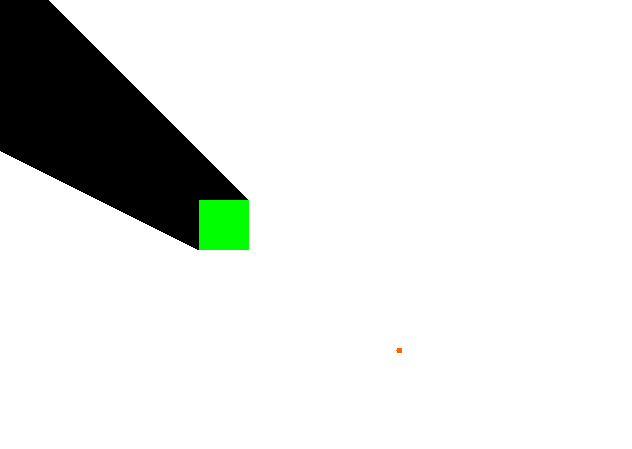
\includegraphics[width=\columnwidth]{images/durchfuehrung.png}
	\caption{einfacher Schatten}
	\label{fig:durch1}
\end{figure}

Im Folgenden wird die entwickelte Methode gezeigt um einen Schatten zu berechnen, wie er zum
Beispiel in Abbildung \ref{fig:durch1} zu sehen ist. Um diesen Schatten darstellen zu können,
werden nun zuerst die zwei Strahlen durch Eckpunkte des schattenwerfenden Objektes berechnet,
die den größten Winkel zueinander haben.

\begin{figure}[t]
	\centering
	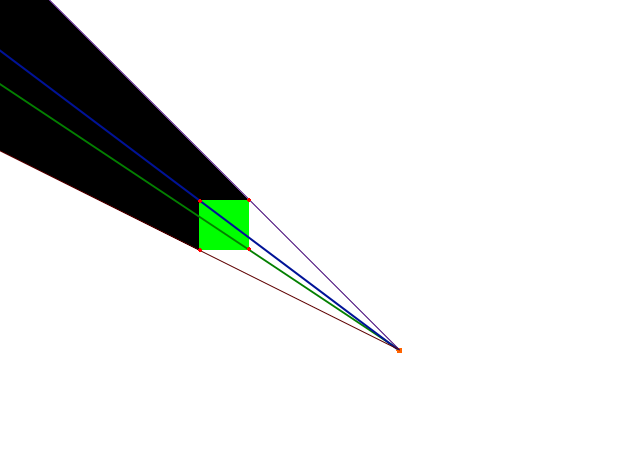
\includegraphics[width=\columnwidth]{images/durchfuehrung_1.png}
	\caption{Geraden durch Eckpunkte}
	\label{fig:durch2}
\end{figure}

Im ersten Schritt der Berechnung werden durch jeden Eckpunkt

\begin{equation}
	P = \begin{pmatrix} p_1 \\ p_2 \end{pmatrix}
\end{equation}

des schattenwerfenden Objektes und die Position der Lichtquelle

\begin{equation}
	L = \begin{pmatrix}  l_1 \\ l_2 \end{pmatrix}
\end{equation}

Geraden mit der Position des Eckpunktes als Ortsvektor und die Position der Lichtquelle subtrahiert
von der Position des Eckpunktes als Richtungsvektor
\begin{equation}
	\vec{g} = \begin{pmatrix} p_1 \\ p_2 \end{pmatrix} + r \cdot \begin{pmatrix} p_1 - l_1 \\ p_2 - l_2 \end{pmatrix}
\end{equation}
gelegt (Abbildung \ref{fig:durch2}).

\begin{figure}[t]
	\centering
	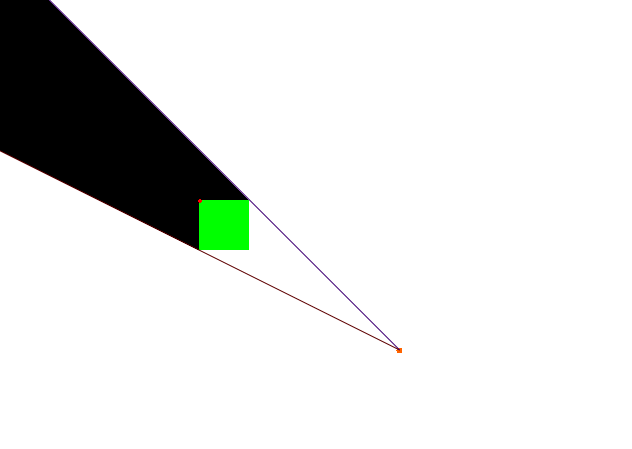
\includegraphics[width=\columnwidth]{images/durchfuehrung_4.png}
	\caption{Geraden mit größtem Winkel}
	\label{fig:durch3}
\end{figure}

Ausschlaggebend für die Silhouette des geworfenen Schatten sind die zwei Geraden, deren Winkel am
weitesten auseinander liegt (Abbildung \ref{fig:durch3}). Um diese zu bestimmen wird rekursiv jedes
Geradenpaar

\begin{equation}
  \begin{split}
	\vec{g}_1 = \vec{o}_1 + r \cdot \vec{m}_1 \\
	\vec{g}_2 = \vec{o}_2 + s \cdot \vec{m}_2
  \end{split}
\end{equation}

durch den Winkel zwischen den beiden Richtungsvektoren der Geraden

\begin{equation}
	\omega = \arccos{\left(\frac{\vec{m}_1 \cdot \vec{m}_2}{|\vec{m}_1| \cdot |\vec{m}_2|} \right)}
\end{equation}

mit dem vorherigen Geradenpaar mit dem größten Winkel zueinander verglichen und das Geradenpaar mit
dem größeren Winkel zueinander zurückgegeben.

\begin{figure}[t]
	\centering
	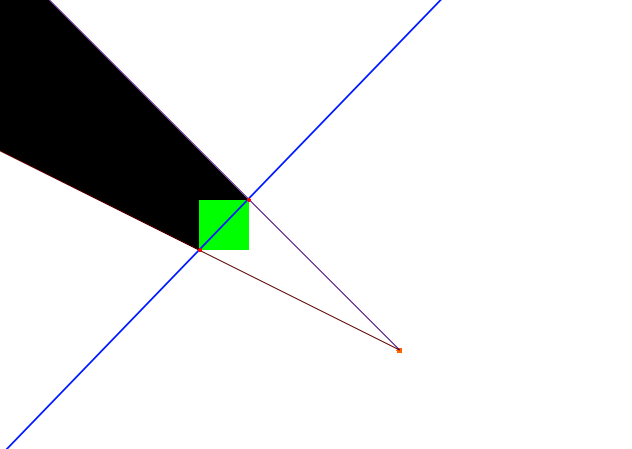
\includegraphics[width=\columnwidth]{images/durchfuehrung_2.png}
	\caption{Gerade durch Ortsvektoren}
	\label{fig:durch4}
\end{figure}

Damit später die Objekte nicht vom eigenen Schatten teilweise bis ganz überdeckt werden, werden nun die Eckpunkte des Rechtecks berechnet, welche auf der unbeleuchteten Seite des Objektes liegen. Dazu wird eine Gerade durch die Ortsvektoren der zwei vorher bestimmten Geraden erzeugt (Abbildung \ref{fig:durch4}).

\begin{equation}
	s: \vec{s} = \vec{o}_1 + t \cdot \left(\vec{o_2} - \vec{o_1}\right)
\end{equation}

\begin{figure}[t]
	\centering
	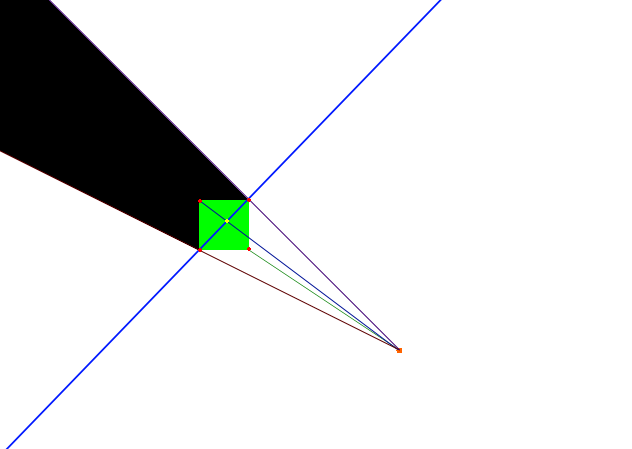
\includegraphics[width=\columnwidth]{images/durchfuehrung_3.png}
	\caption{Eckpunkte auf der dunklen Seite}
	\label{fig:durch5}
\end{figure}

Wenn ein Schnittpunkt zwischen der Geraden $s$ und der Strecke zwischen einem Eckpunkt des Rechtecks
und der Position der Lichtquelle vorhanden ist hängen wir diesen Eckpunkt an das an den Rasterizer
zu übergebende Array von Punkten an (Abbildung \ref{fig:durch5}).

Durch die Arbeitsweise des Rasterizers müssen die Schnittpunkte der zwei Silhouettenstrahlen mit den
Fenstergrenzen nicht berechnet werden. Dieses Schattenmodell, bestehend aus zwei Strahlen und einem
Array an Punkten, kann an den Rasterizer übergeben werden.

Der Rasterizer wendet dieses Konstrukt mit Hilfe des aktive Kantenlisten Algorithmus auf die
Lichtwerte der Pixel in der Szene an. Der aktive Kantenlisten Algorithmus erlaubt eine inkrementelle
Berechnung der Schnittpunkte zwischen Polygonkanten und Pixelzeilen und somit ob ein Pixel
im Polygon liegt und eingefärbt wird oder nicht. Dazu wird eine Tabelle erzeugt, die für jede Pixelzeile eine Liste an aktiven Kanten
enthält. Diese aktiven Kanten enthalten die x-Koordinate $x$ des Schnittpunktes mit der aktuellen Bildzeile, die
Differenz zwischen den x-Koordinaten der Schnittpunkte $\Delta x$ zweier vertikal benachbarter
Geraden und die Anzahl der Bildzeilen $n_y$, die von der Polygonkante noch geschnitten werden. Nun
werden die Bildzeilen inkrementell durchlaufen. Dabei werden die Kanten in einer Bildzeile nach $x$
des Schnittpunktes aufsteigend geordnet. Dann wird von $x$ der ersten Kante bis $x$ der zweiten Kante in der Liste
jedes Pixel eingefärbt. Diese beiden Kanten werden inkrementiert und die nächsten beiden Kanten werden
betrachtet, bis keine Kanten mehr in der Bildzeile übrig sind. Dann wird die nächste Bildzeile
nach dem selben Schema behandelt. Eine Kante wird inkrementiert indem die Kante in die nächsthöhere Bildzeile verschoben
wird, $x$ auf $x + \Delta x$ gesetzt und $n_y$ dekrementiert wird.


Durch die Beschaffenheit dieses Algorithmus wird für den übergebenen Schatten in vielen Fällen nicht das komplette
Polygon ausgerechnet.
